\section{Queueing networks}

Queueing theory studies the behavior of systems with numerous tasks and limited resources, leading to queues and delays. 
It models computer systems as networks of queues.
\begin{definition}[\textit{Queueing networks}]
    A network of queues consists of service centers (system resources) and customers (users or transactions).
\end{definition}

In computer systems, queues are prevalent:
\begin{itemize}
    \item The CPU uses a time-sharing scheduler.
    \item Disk operations involve a queue of requests waiting for block reads or writes.
    \item Routers manage queues of packets awaiting routing.
    \item Databases feature lock queues, where transactions wait for record locks.
\end{itemize}
Queueing theory aids in performance prediction, particularly for capacity planning, and relies on stochastic modeling and analysis.
The success of queueing networks lies in their ability to abstract low-level system details, focusing instead on high-level performance characteristics.

\paragraph*{Single queue}
In a single queue scenario, customers from a certain population arrive at a service facility.
This facility, equipped with one or more servers, provides the required service to customers.
If a customer cannot access a server immediately, they join a queue or buffer until a server becomes available. 
Upon completion of service, the customer departs, and the server selects the next customer from the buffer based on the service discipline or queuing policy.

\subsection{Queueing model}
The elements of queueing models are:
\begin{itemize}
    \item \textit{Arrival of customers}: customer arrivals represent jobs entering the system, detailing their frequency, speed, and types. 
        \begin{figure}[H]
            \centering
            \begin{subfigure}{0.32\textwidth}
                \centering
                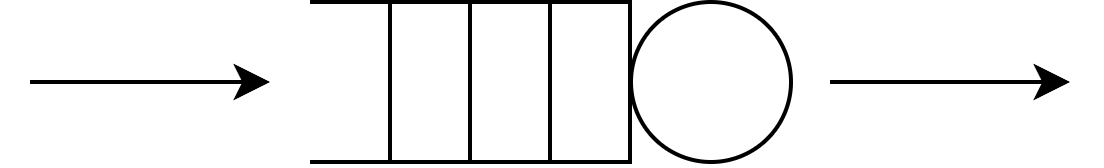
\includegraphics[width=1\linewidth]{images/ext.png} 
                \caption{Data from external source}
            \end{subfigure}
            \begin{subfigure}{0.32\textwidth}
                \centering
                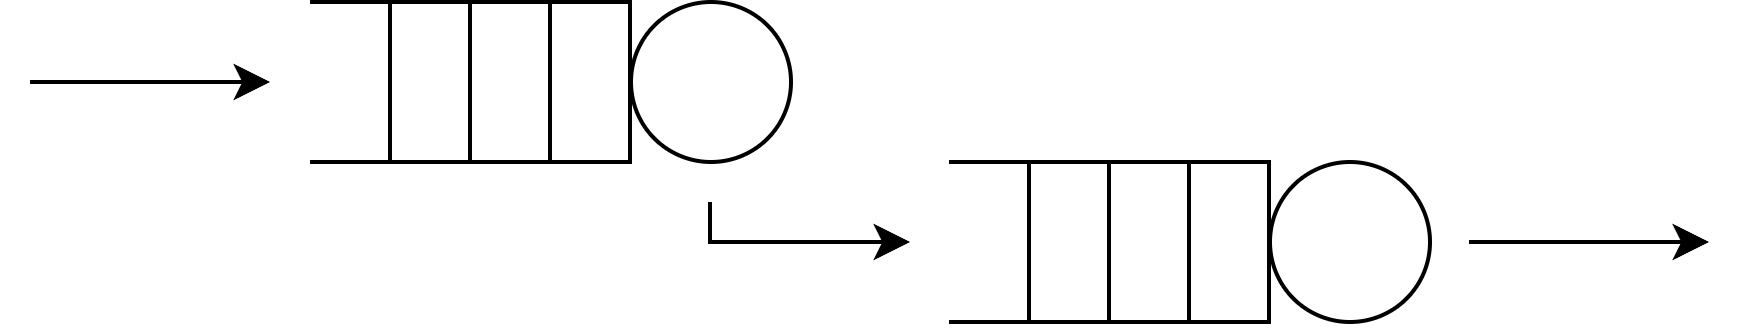
\includegraphics[width=1\linewidth]{images/ext1.png} 
                \caption{Data from another queue}
            \end{subfigure}
            \begin{subfigure}{0.32\textwidth}
                \centering
                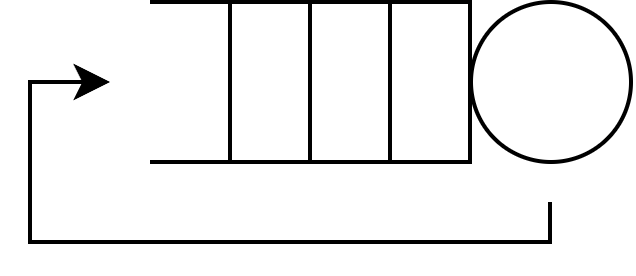
\includegraphics[width=0.6\linewidth]{images/ext2.png}
                \caption{Data from same queue}
            \end{subfigure}
            \caption{Types of data arrival}
        \end{figure}
    \item \textit{Service}: he duration a job spends being served, indicating the time a server dedicates to satisfying a customer.
        The key characteristics of service time include its average duration and distribution function. 
        Possible scenarios include:
        \begin{itemize}
            \item \textit{Single server}: the service facility can handle only one customer at a time.
                Waiting customers remain in the queue until selected for service, with the selection process depending on the service discipline.
            \item \textit{Multiple servers}: a fixed number of servers, each capable of serving a customer simultaneously. 
                If the number of customers is less than or equal to the number of servers, there is no queueing, and each customer has direct access to a server. 
                Otherwise, additional customers must wait in the queue.
            \item \textit{Infinite servers}: there are always enough servers available for every arriving customer, eliminating queues.
        \end{itemize}
    \item \textit{Queue}: if the number of jobs exceeds the system's parallel processing capacity, they queue in a buffer. 
        Customers unable to receive immediate service wait in the buffer until a server becomes available. 
        When the buffer reaches its finite capacity, two options arise:
        \begin{itemize}
            \item The facility being full is communicated to the arrival process, suspending arrivals until capacity is available, or a customer leaves.
            \item Arrivals continue, but incoming customers are turned away until capacity is available again.
        \end{itemize}
        When a job in service leaves the system, a job from the queue can enter the now vacant service center. 
        The queuing policy dictates which job in the queue starts its service. 
        In cases where multiple customers are waiting, a rule determines which waiting customer gains access to a server next. 
        Common service disciplines include FIFO, LIFO, random selection, and priority.
    \item \textit{Population}: the characteristic of interest regarding the population is typically its size.
        If the population size is fixed, no more than $N$ customers will ever require service simultaneously. 
        When the population is finite, the arrival rate of customers is influenced by the number already in the service facility.
        If the population size is so large that it has no noticeable impact on the arrival process, it is assumed to be infinite. 
        Users can be categorized based on their behaviors, with different classes differing in characteristics such as arrival rate or service demand.
    \item \textit{Routing}: when a job completes service at a station and has multiple potential routes, a suitable selection policy must be established. 
        This policy, dictating how the next destination is chosen, is termed routing.
        The main routing algorithms include probabilistic (each path is assigned a probability), round robin (job rotation among all paths), and shortest queue (path with the least occupied queue).
\end{itemize}
For many systems, the system can be conceptualized as a collection of resources and devices, with customers or jobs circulating among them. 
Each resource in the system can be associated with a service center, and customers are routed among these service centers.
After receiving service at one service center, a customer may move on to other service centers based on a predefined pattern of behavior corresponding to the customer's requirements.

\subsection{Taxonomy}
A queueing network can be depicted as a graph, where nodes represent the service centers and arcs signify potential transitions of users from one service center to another.
Together, nodes and arcs define the network's topology.
\begin{figure}[H]
    \centering
    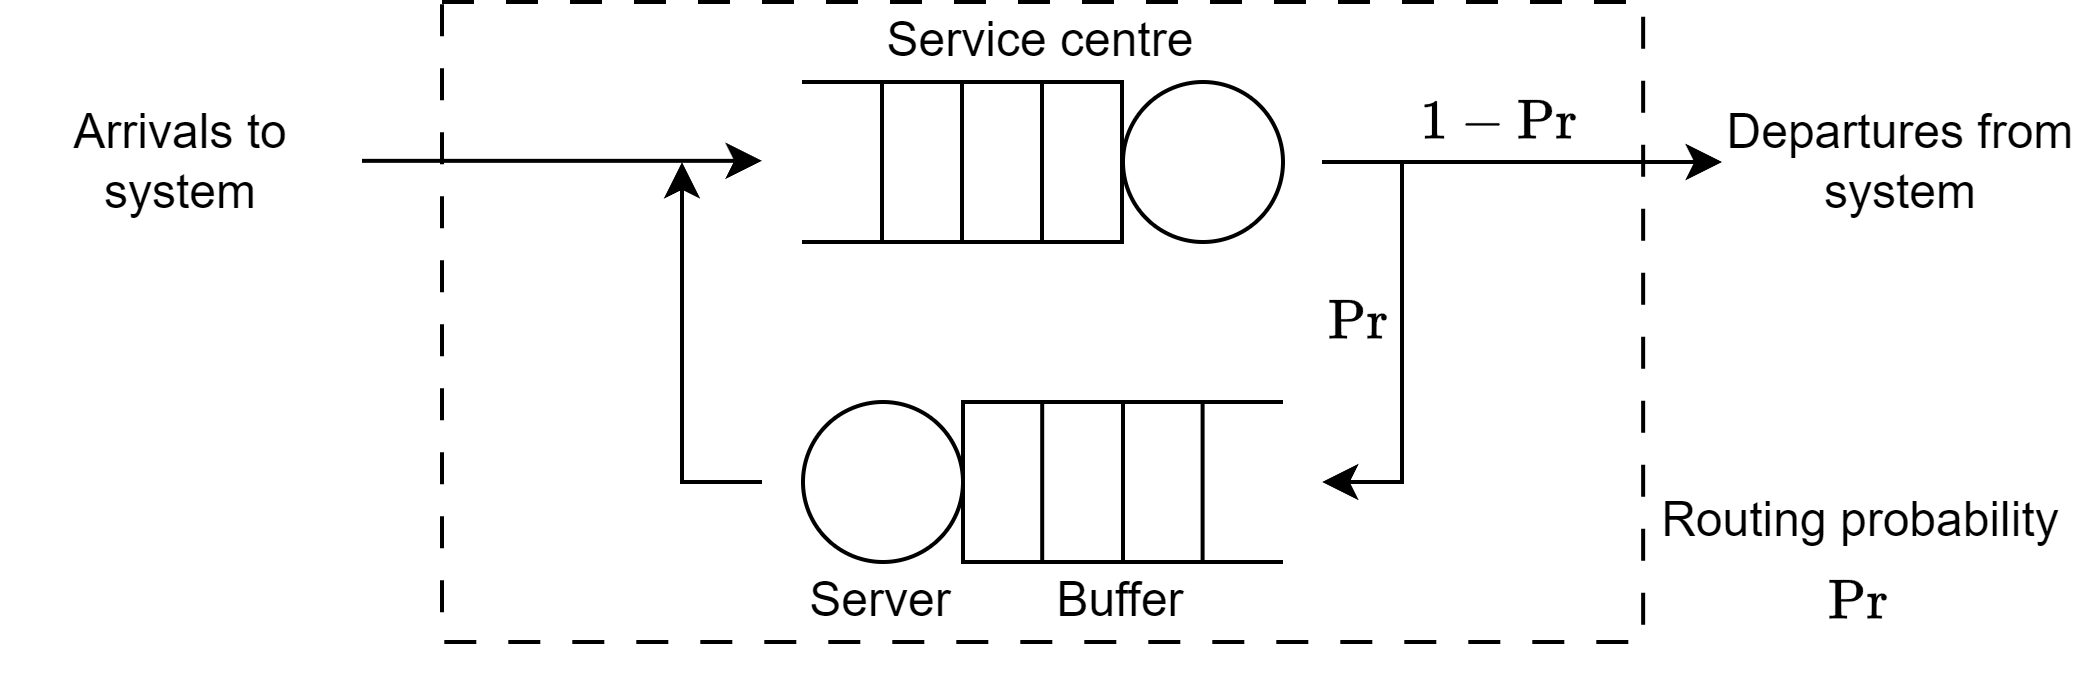
\includegraphics[width=0.65\linewidth]{images/per.png}
    \caption{Queueing network representation}
\end{figure}
A network may be:
\begin{itemize}
    \item \textit{Open}: customers may arrive from or depart to some external environment.
    \item \textit{Closed}: a fixed population of customers remains within the system.
    \item \textit{Mixed}: classes of customers within the system exhibit both open and closed patterns of behavior.
\end{itemize}

\begin{figure}[H]
    \centering
    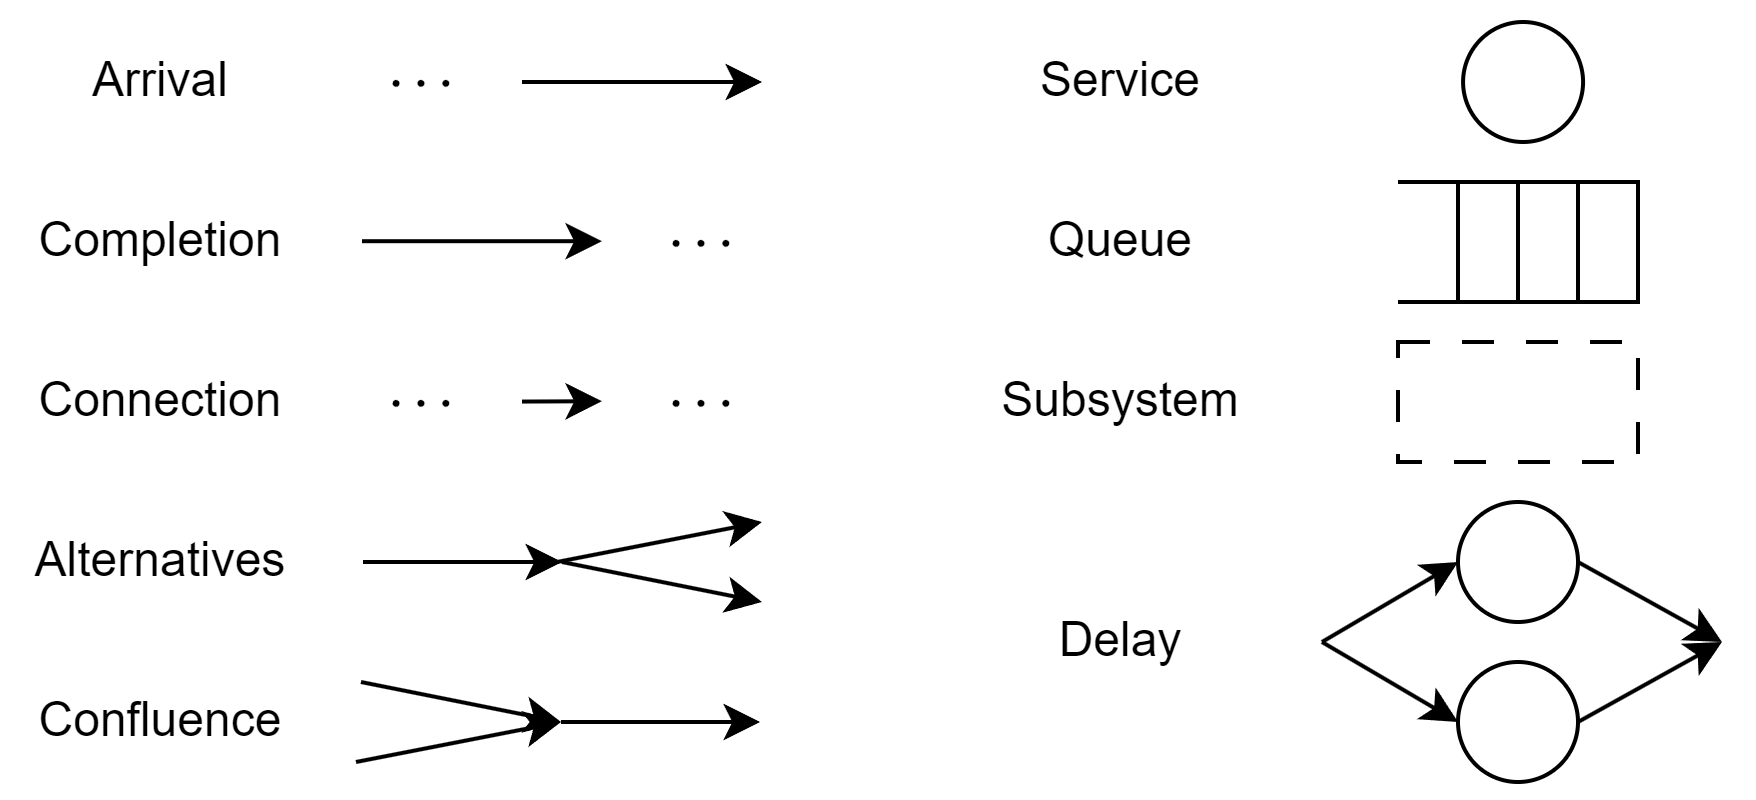
\includegraphics[width=0.75\linewidth]{images/gra.png}
    \caption{Graphical notation}
\end{figure}